\section{Experiments}
%\bing{图表在论文中的位置，原则上尽量贴近主要讨论他们的文本部分，最后排版的时候注意一下}
We evaluate EverMemOS on two long-horizon memory-augmented reasoning benchmarks (LoCoMo~\cite{maharana2024locomo} and LongMemEval~\cite{wu2025long}), and report a profile study on PersonaMem-v2~\cite{jiang2025personamem}.

\subsection{Experimental Setup}

\paragraph{Benchmarks}
We evaluate memory-augmented reasoning on LoCoMo and LongMemEval. LoCoMo contains 1{,}540 questions over 10 ultra-long dialogues ($\sim$9K tokens each), spanning single-hop, multi-hop, and temporal questions. LongMemEval (S-setting, $\sim$115k tokens per conversation) evaluates 500 questions requiring full-history parsing across core capabilities (e.g., updates and abstention). We additionally evaluate user profiling on PersonaMem-v2.

\paragraph{Baselines}
We compare EverMemOS against state-of-the-art memory systems: \textbf{Zep} \cite{zep2025}, \textbf{Mem0} \cite{mem02025}, \textbf{MemOS} \cite{li2025memos}, \textbf{MemoryOS} \cite{kang2025memory}, and \textbf{MemU}\footnote{Open-source memory infrastructure: \url{https://github.com/NevaMind-AI/memU}}.
\textbf{Fair comparison:} We standardize the answer-generation backbone across methods while keeping each baseline's official memory configuration unchanged; for LongMemEval, we report baseline scores from the official \textbf{MemOS} leaderboard. Full settings are provided in Appendix~\ref{sec:eval_setting}.

\paragraph{Evaluation Protocol}
We adopt the \textbf{LLM-as-a-judge} protocol, following MemOS: each answer is evaluated by GPT-4o-mini and two auxiliary judge models, and scores are averaged across the three judgments in a \emph{blind} setting. We validate the reliability of this protocol against human annotations in Section~\ref{sec:judge_reliability} (Appendix), showing high agreement (Cohen's $\kappa > 0.89$).


\paragraph{Implementation Details}
EverMemOS uses GPT-4.1-mini (or GPT-4o-mini where specified) for all reasoning and memory operations. Retrieval uses hybrid dense+BM25 fusion (RRF) with re-ranking. Default retrieval hyperparameters are in Appendix~\ref{sec:eval_setting}. Unless otherwise specified, quantitative experiments use \textbf{Memory-Augmented Reasoning}.
We provide a token-level cost breakdown by lifecycle phase in Appendix (Table~\ref{tab:token_cost}).

\subsection{Main Results}

\begin{table*}[!h]
\centering
\small
\setlength{\tabcolsep}{5pt}
\begin{tabular}{l r ccccc}
\toprule
\textbf{Method} & \textbf{Avg. Tokens} & \textbf{Single Hop} & \textbf{Multi Hop} & \textbf{Temporal} & \textbf{Open Domain} & \textbf{Overall} \\
\midrule
\multicolumn{7}{l}{\textit{GPT-4o-mini backbone}} \\[-2pt]
MemoryOS & 5.2k & 62.43 & 56.50 & 37.18 & 40.28 & 54.70 \\
Mem0 & 1.0k & 66.71 & 58.16 & 55.45 & 40.62 & 61.00 \\
MemU & 4.0k & 72.77 & 62.41 & 33.96 & 46.88 & 61.15 \\
MemOS & 2.5k & 81.45 & 69.15 & 72.27 & 60.42 & 75.87 \\
Zep & 1.4k & 88.11 & 71.99 & 74.45 & 66.67 & 81.06 \\
\textbf{EverMemOS} & 2.5k & \textbf{91.08} {\scriptsize ($\uparrow$3.4\%)} & \textbf{86.17} {\scriptsize ($\uparrow$19.7\%)} & \textbf{81.93} {\scriptsize ($\uparrow$10.0\%)} & \textbf{66.67} {\scriptsize ($\uparrow$0.0\%)} & \textbf{86.76} {\scriptsize ($\uparrow$7.0\%)} \\

\midrule
\multicolumn{7}{l}{\textit{GPT-4.1-mini backbone}} \\[-2pt]
MemoryOS & 5.5k & 67.30 & 59.34 & 42.26 & 59.03 & 60.11 \\
Mem0 & 1.0k & 68.97 & 61.70 & 58.26 & 50.00 & 64.20 \\
MemU & 4.0k & 74.91 & 72.34 & 43.61 & 54.17 & 66.67 \\
MemOS & 2.5k & 85.37 & 79.43 & 75.08 & 64.58 & 80.76 \\
Zep & 1.4k & 90.84 & 81.91 & 77.26 & 75.00 & 85.22 \\
\textbf{EverMemOS} & 2.3k & \textbf{96.67} {\scriptsize ($\uparrow$6.4\%)} & \textbf{91.84} {\scriptsize ($\uparrow$12.1\%)} & \textbf{89.72} {\scriptsize ($\uparrow$16.1\%)} & \textbf{76.04} {\scriptsize ($\uparrow$1.4\%)} & \textbf{93.05} {\scriptsize ($\uparrow$9.2\%)} \\
\bottomrule
\end{tabular}
\caption{Main results on \textbf{LoCoMo} under two backbones. All metrics are accuracy (\%), except Avg. Tokens. For EverMemOS, values in parentheses denote relative change (\%) compared to the strongest baseline under the same backbone.}
\label{tab:locomo-main}
\end{table*}
\begin{table*}[!h]
    \centering
    \small
    \setlength{\tabcolsep}{2pt}
    \begin{tabular}{@{}l c ccccccc@{}}
    \toprule
    \textbf{Method} & \textbf{Token} & \textbf{SS-User} & \textbf{SS-Asst} & \textbf{SS-Pref} & \textbf{Multi-S} & \textbf{Know. Upd} & \textbf{Temp. Reas} & \textbf{Overall} \\
    \midrule
    MemU & 0.5k & 67.14 & 19.64 & 76.67 & 42.10 & 41.02 & 17.29 & 38.40 \\
    Zep & 1.6k & 92.90 & 75.00 & 53.30 & 47.40 & 74.40 & 54.10 & 63.80 \\
    Mem0 & 1.1k & 82.86 & 26.78 & 90.00 & 63.15 & 66.67 & 72.18 & 66.40 \\
    MemOS & 1.4k & 95.71 & 67.86 & \textbf{96.67} & 70.67 & 74.26 & \textbf{77.44} & 77.80 \\
    \textbf{EverMemOS} & 2.8k & \textbf{97.14} {\tiny ($\uparrow$1.5\%)} & \textbf{85.71} {\tiny ($\uparrow$14.3\%)} & 93.33 {\tiny ($\downarrow$3.5\%)} & \textbf{73.68} {\tiny ($\uparrow$4.3\%)} & \textbf{89.74} {\tiny ($\uparrow$20.6\%)} & \textbf{77.44} {\tiny ($\uparrow$0.0\%)} & \textbf{83.00} {\tiny ($\uparrow$6.7\%)} \\
    \bottomrule
    \end{tabular}
    \caption{Main results on \textbf{LongMemEval} (accuracy, \%). SS denotes single-session tasks; baselines are from the official \textbf{MemOS} results \cite{li2025memos}. For EverMemOS, values in parentheses denote relative change (\%) compared to the strongest baseline for that metric.}
    \label{tab:longmemeval-main}
\end{table*}

Main results on two benchmarks are reported in Tables~\ref{tab:locomo-main}-\ref{tab:longmemeval-main}. We make three observations:

(1) \textbf{Lifecycle-driven performance gains.}
EverMemOS outperforms the strongest baseline on each benchmark overall, i.e., Zep on LoCoMo by 7.0\% and 9.2\%, and MemOS on LongMemEval by 6.7\%.
%
We attribute this to the shift from flat memory storage to a structured lifecycle, which consolidates fragmented experiences into usable knowledge before retrieval, providing a more robust context than isolated record matching. 


(2) \textbf{Structural consolidation aids complex reasoning that requires integrating dispersed evidence.}
%Improvements are most pronounced on multi-hop or temporal questions in LoCoMo and on knowledge update or SS-Asst in LongMemEval, while open domain remains comparable to Zep. 
% \bing{对两个benchmarks的评测维度，写法要一直，比如首字母大小写、是否加粗}\
We can observe significant gains on LoCoMo multi-hop (+19.7\%) and temporal (+10.0\%) tasks, as well as LongMemEval knowledge update (+20.6\%), validating the effectiveness of MemScenes. By clustering related episodes into coherent thematic units, EverMemOS presents the solver with a complete narrative context. This enables LLMs to naturally bridge dispersed evidence and resolve state conflicts that confuse other models relying on fragmented retrieval.

(3) \textbf{EverMemOS offers a favorable accuracy-efficiency trade-off.}
%Figure~\ref{fig:frontier} shows that EverMemOS attains high accuracy with moderate retrieval budgets, suggesting that improvements come from composing necessary and sufficient evidence rather than overly expanding context.
%
%\textbf{Precision via Reconstructive Recollection.} EverMemOS offers a favorable accuracy-efficiency trade-off. 
As shown in Figure~\ref{fig:frontier} , EverMemOS attains high accuracy with moderate retrieval budgets. This efficiency confirms the utility of the Reconstructive Recollection phase, where the agentic sufficiency check ensures the context is composed of necessary and sufficient evidence, avoiding the noise accumulation common in fixed-budget retrieval.

\subsection{Ablation Study}
\label{sec:ablation}
We conduct ablations on LoCoMo to isolate the contributions of \textit{MemScenes}, \textit{MemCells}, and episode segmentation.

\begin{figure}[t]
    \centering
    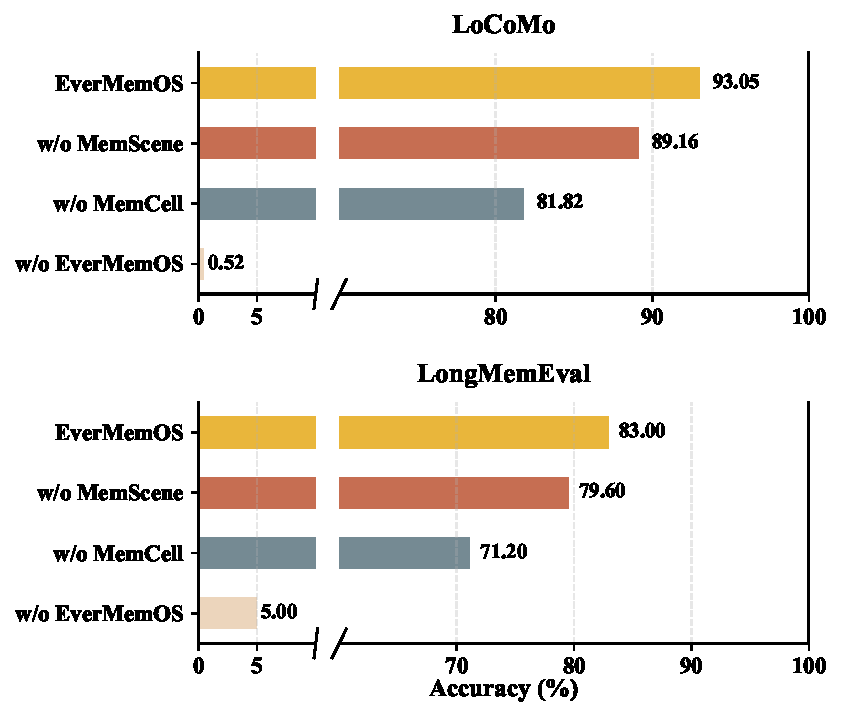
\includegraphics[width=0.95\linewidth]{figure/ablation_overall.pdf}
    \vspace{-2mm}
    \caption{Ablation results (overall accuracy) on LoCoMo and LongMemEval.}
    \vspace{-4mm}
    \label{fig:ablation_chart}
\end{figure}

\begin{figure}[t]
    \centering
    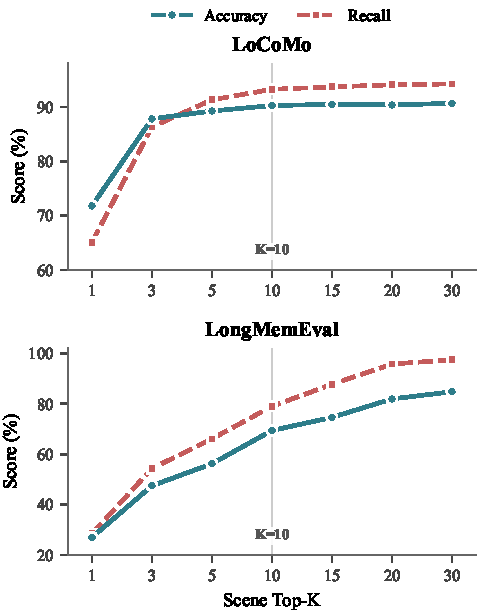
\includegraphics[width=0.9\linewidth]{figure/hyperpara.pdf}
    \vspace{-2mm}
    \caption{Sensitivity analysis on the MemScene count ($N$).}
    \vspace{-4mm}
    \label{fig:hyperpara}
\end{figure}


\begin{figure}[t]
    \centering
    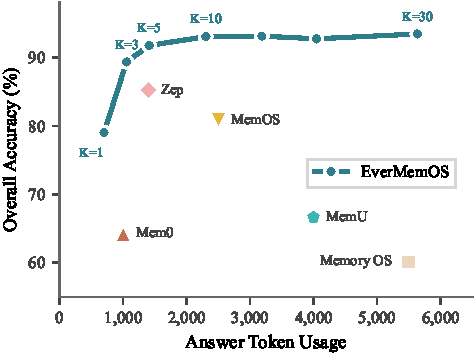
\includegraphics[width=0.9\linewidth]{figure/efficiency_tradeoff.pdf}
    \vspace{-2mm}
    \caption{Performance vs. cost frontier on LoCoMo by varying the retrieved episode count ($K$).}
    \vspace{-4mm}
    \label{fig:frontier}
\end{figure}

\begin{figure*}[t]
    \centering
    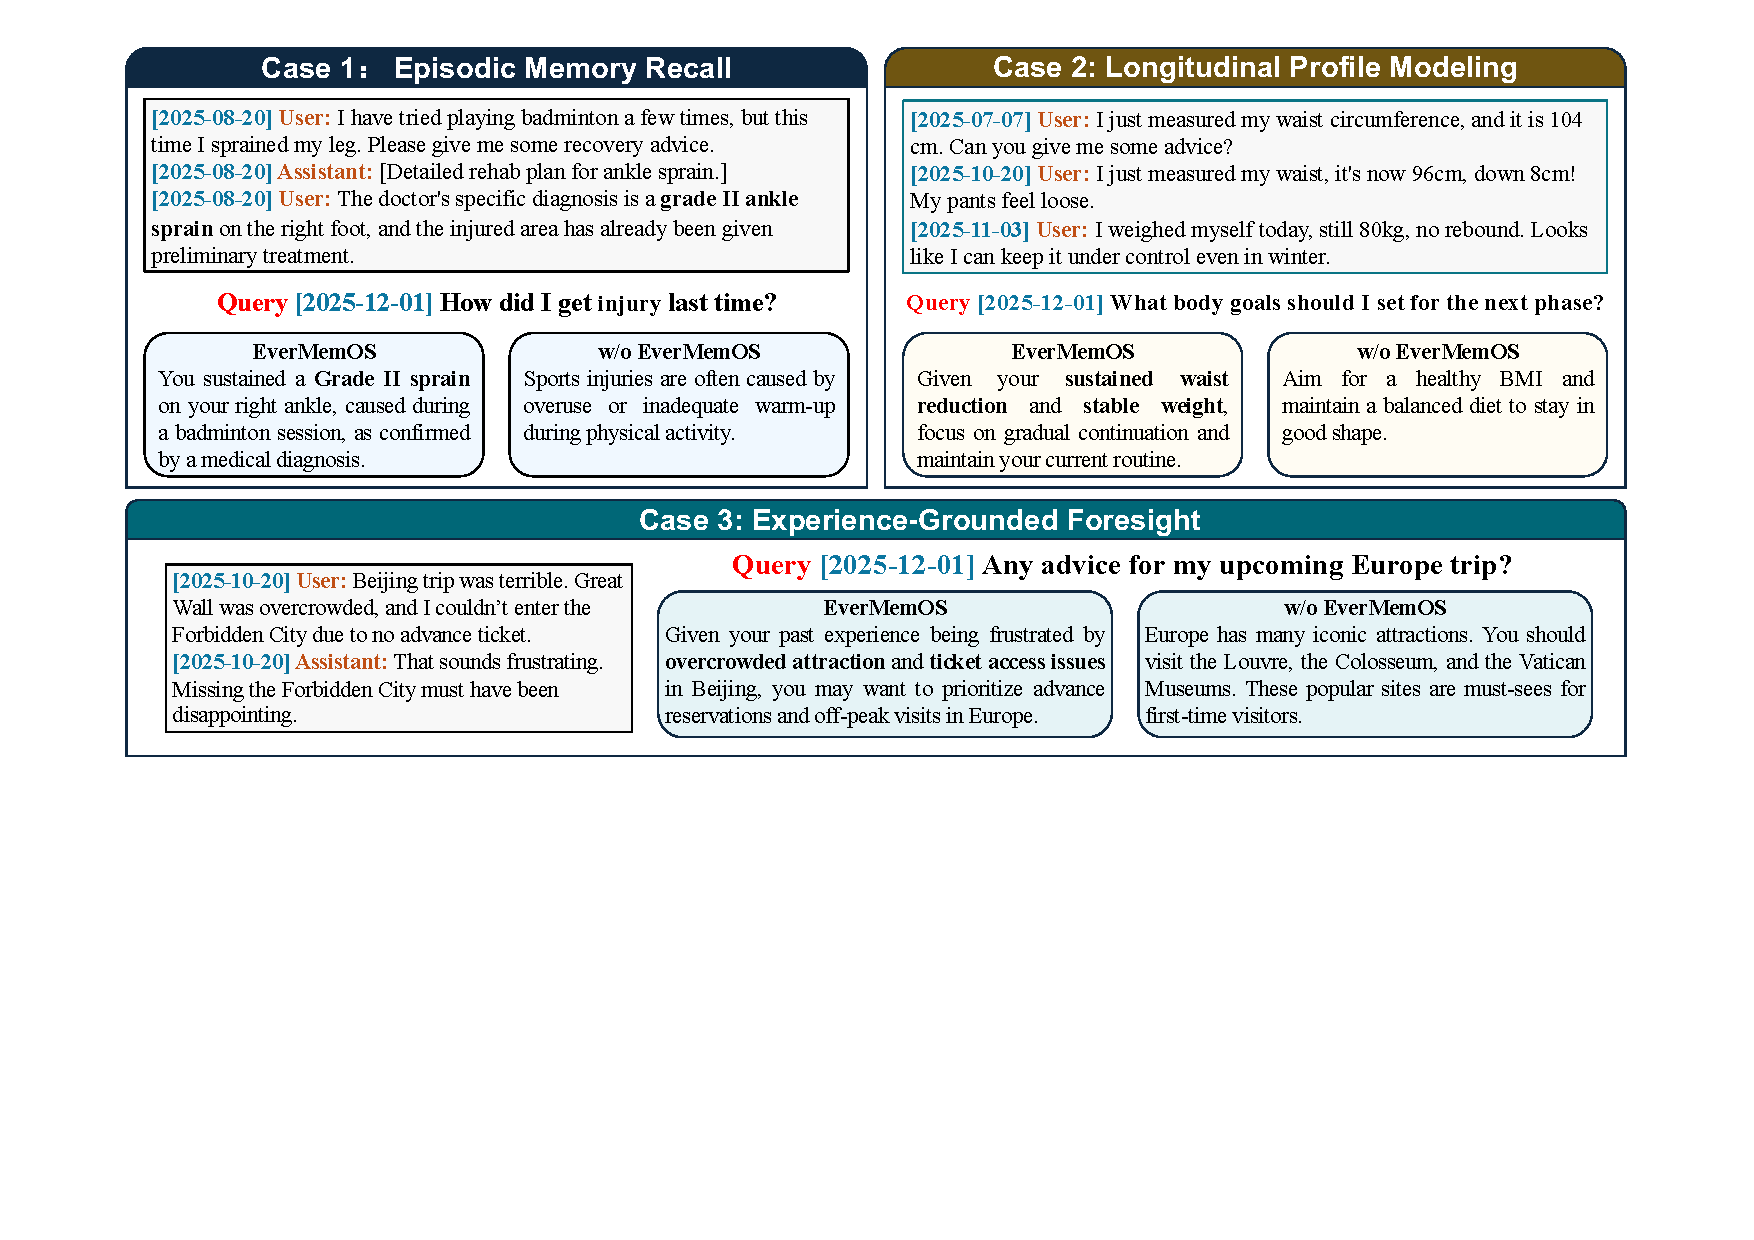
\includegraphics[width=0.9\linewidth]{figure/case.pdf}
    \vspace{-2mm}
    \caption{Case studies illustrating Profile, Foresight, and Episode capabilities in Memory-Augmented Chat.}
    \vspace{-2mm}
    \label{fig:case_study}
\end{figure*}

\textbf{Impact of Memory Architecture.} 
To isolate the contribution of memory structure, we compare EverMemOS with three degraded variants: w/o EverMemOS (no external memory), w/o MemScene (flat retrieval over MemCells), and w/o MemCell (retrieval over raw dialogue). The backbone model and prompts are fixed, and only the memory representation and retrieval pipeline are varied.

As shown in Figure~\ref{fig:ablation_chart}, performance degrades stepwise as structure is removed, revealing three corresponding capability losses. Removing \textit{MemScenes} eliminates scene-level organization, weakening cross-turn aggregation over related episodes. Removing \textit{MemCells} further drops the stable semantic units (episodes/facts), forcing retrieval to rely on raw dialogue matching. Finally, removing external memory collapses long-horizon performance, indicating that many queries cannot be handled reliably within the context window alone.

\textbf{Effectiveness of Episode Segmentation.} 
We evaluate semantic episode segmentation against fixed heuristics and ground-truth boundaries under \textbf{w/o MemScene} to isolate boundary quality.
%
We compare three strategies: (1) \textbf{Fixed Heuristics} (fixed message count $N=10$ or token thresholds $N=512,1024$); (2) \textbf{Session (Oracle)} (ground-truth session boundaries); and (3) \textbf{EverMemOS} (semantic segmentation with different backbones).

\begin{table}[!t]
    \centering
    \small
    \renewcommand{\arraystretch}{1.15}
    \setlength{\tabcolsep}{5pt}
    
    \begin{tabular}{l c c}
        \toprule
        & \multicolumn{2}{c}{\textbf{Answer Model}} \\
        \cmidrule(lr){2-3}
        \textbf{Segmentation Method} & \textbf{GPT-4.1-mini} & \textbf{Qwen3-4B} \\
        \midrule
        \multicolumn{3}{l}{\textit{Heuristic Baselines}} \\
        Fixed-Message-10 & 88.05 & 80.95 \\
        Fixed-Token-512 & 87.55 & 80.67 \\
        Fixed-Token-1024 & 84.52 & 75.19 \\
        \midrule
        \multicolumn{3}{l}{\textit{Semantic Segmentation}} \\
        Session (Oracle) & 87.66 & 80.63 \\
        \textbf{Default (EverMemOS)} &  &  \\
        $\quad$ w/ GPT-4.1-mini & 89.16 & 83.07 \\
        $\quad$ w/ Qwen3-4B & 89.78 & 82.73 \\
        \bottomrule
    \end{tabular}
    \vspace{-2mm}
    \caption{
        Comparison of boundary detection strategies.
        \textbf{Session (Oracle)} uses the ground-truth session partitions provided by LoCoMo.
    }
    \vspace{-4mm}
    \label{tab:locomo-bound}
\end{table}

Table~\ref{tab:locomo-bound} shows that (i) semantic segmentation consistently outperforms fixed heuristics, especially coarse token chunking; (ii) it also outperforms Session (Oracle), suggesting sessions are not always optimal retrieval units; and (iii) results are robust across boundary-detection backbones (accuracy changes $\leq$0.7 points).

\subsection{Hyperparameter Analysis}
\label{sec:sensitivity}
We investigate the impact of retrieval scope via two hyperparameters: the number of retrieved \textit{MemScenes} ($N$) and episodes ($K$). As shown in Figure~\ref{fig:hyperpara}, performance gains saturate around $N=10$. Figure~\ref{fig:frontier} further illustrates the efficiency--accuracy frontier governed by $K$. We therefore adopt $N=10$ and $K=10$ as the default configuration to balance performance with computational cost. Comprehensive sensitivity analysis is detailed in Appendix~\ref{sec:sensitivity_details}.


\subsection{Profile Study}
\label{sec:profile_study}
\begin{table}[t]
    \centering
    \small
    \setlength{\tabcolsep}{3pt}
    \renewcommand{\arraystretch}{1.0}
    \begin{tabular}{l r r r}
    \toprule
    \textbf{Scenario} & \textbf{Ep.+Prof.} & \textbf{Prof.-only} & \textbf{Ep.-only} \\
    \midrule
Consultation        & \textbf{51.03} & 47.33 & 44.44 \\
Email (Personal)    & \textbf{53.85} & 46.15 & 46.15 \\
Translation         & \textbf{50.00} & 46.15 & 38.08 \\
Email (Professional) & \textbf{53.79} & 41.38 & 45.17 \\
Writing (Creative)    & \textbf{55.10} & 48.57 & 42.04 \\
Writing (Professional) & \textbf{45.56} & 44.79 & 40.15 \\
Knowledge Query     & \textbf{63.68} & 62.94 & 54.73 \\
Social Media        & \textbf{47.90} & 44.96 & 36.13 \\
Chat                & \textbf{52.09} & 44.87 & 41.83 \\
\midrule
\textbf{Overall}    & \textbf{53.25} & 48.30 & 43.93 \\
    \bottomrule
    \end{tabular}
    %\vspace{-2mm}
    \caption{Profile ablation on PersonaMem v2~\cite{jiang2025personamem} (5{,}000 questions across 9 scenarios; accuracy, \%).}
    \vspace{-2mm}
    \label{tab:profile_effect}
    \end{table}
We evaluate the effect of the consolidated user profile on PersonaMem-v2 (32k)~\cite{jiang2025personamem}; results are not directly comparable across dataset versions due to differences in task setup and annotations. Table~\ref{tab:profile_effect} shows that adding the User Profile to episodic evidence improves overall accuracy by 9.32 points over episodes-only (53.25 vs.\ 43.93), indicating that semantic consolidation provides complementary signal beyond episodic retrieval. We defer the full comparison against other memory systems on PersonaMem-v2 to Appendix~\ref{sec:personamem_full}.

\subsection{Case Study}
Existing benchmarks primarily evaluate answer-level accuracy/recall and do not capture several capabilities required for long-term conversational agents, such as conflict detection, profile stability, and experience-grounded foresight. To complement quantitative results, Figure~\ref{fig:case_study} shows three representative cases: \textbf{(Episode)} reconstructing a concrete past injury episode (a Grade-II ankle sprain during badminton) rather than producing a generic explanation; \textbf{(Profile)} maintaining longitudinal stability and using sustained improvements (waist 104$\rightarrow$96\,cm with stable weight) for trajectory-consistent goal setting; and \textbf{(Foresight)} leveraging previously observed failures (overcrowding and missing advance tickets) to make proactive recommendations for future travel.
Together, these cases illustrate coherent, experience-aware behavior beyond what is measured by existing benchmarks.